
The moment of inertia of the gear train was thoroughly calculated in a previous report and will be used here.

\subsubsection*{Method}
The gear train can by divided in three parts: the large wheels, the small wheels and the axles. The latter is a solid cylinder whereas the wheels are considered as multiple hollowed cylinders. The moment of inertia about a symmetry axis through the center of mass for a hollow cylinder is described in \autoref{eq:MomentInertiaHollowedCylinder}: 
\begin{equation}
	J_{hc} = \frac{1}{2} M (R_1^2 + R_2^2)
	\label{eq:MomentInertiaHollowedCylinder}
\end{equation}
\startexplain
\explain{$J_{hc}$ is the moment of inertia about a symmetry axis through the center of mass for a hollow cylinder}{\si{\kilo\gram\meter\squared}}
\explain{$M$ is the mass of the hollowed cylinder}{\si{\kilo\gram}}
\explain{$R_1$ is the inner radius of the hollowed cylinder}{\si{\meter}}
\explain{$R_2$ is the outer radius of the hollowed cylinder}{\si{\meter}}
\stopexplain

For the axles, the inner radius $R_1$ is equal to zero, giving equation \autoref{eq:MomentInertiaSolidCylinder} for the solid cylinder.
\begin{equation}
	J_{sc} = \frac{1}{2} M R^2
	\label{eq:MomentInertiaSolidCylinder}
\end{equation}
\startexplain
\explain{$J_{sc}$ is the moment of inertia about a symmetry axis through the center of mass for a solid cylinder}{\si{\kilo\gram\meter\squared}}
\explain{$M$ is the mass of the solid cylinder}{\si{\kilo\gram}}
\explain{$R$ is the inner radius of the solid cylinder}{\si{\meter}}
\stopexplain

The mass of each wheels and axles are calculated using their volumes and the density of iron.

\begin{figure}[htbp]
    \centering
    \begin{minipage}[t]{0.45\textwidth}
        \centering
        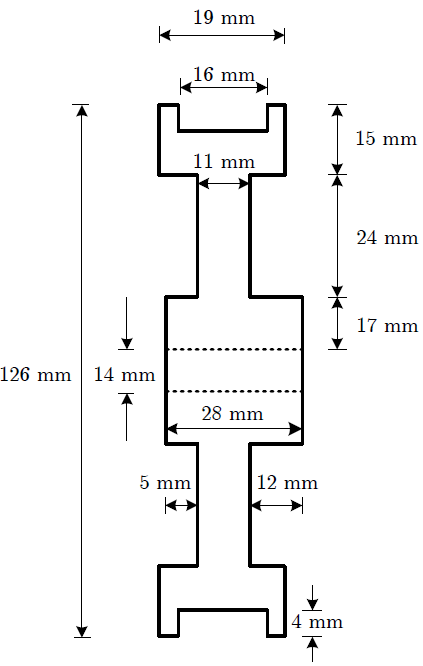
\includegraphics[width=0.9\textwidth]{figures/appendix/Motor&GearTests/BigWheel} 
        \caption{Cross section of a large wheel \citep{web:BalancingStick2008}.}
    \end{minipage}\hfill
    \begin{minipage}[t]{0.45\textwidth}
        \centering
        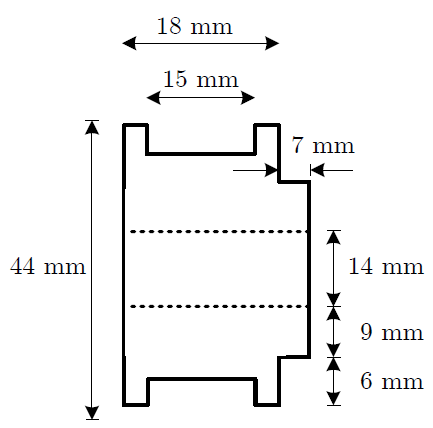
\includegraphics[width=0.9\textwidth]{figures/appendix/Motor&GearTests/SmallWheel} 
        \caption{Cross section of a small wheel \citep{web:BalancingStick2008}.}
    \end{minipage}
\end{figure}

\subsubsection*{Conclusion}
The moment of inertia for each part of the gear system \citep{web:BalancingStick2008}:
\begin{subequations} \label{eq:ResumeMomentInertiaGears}
	\begin{flalign}
		\text{Large Wheel: } J_{Large} &= 1.433 \cdot 10^{-3} \ \si{\kilo\gram\meter\squared} \\
		\text{Small Wheel: } J_{Small} &= 0.037 \cdot 10^{-3}\ \si{\kilo\gram\meter\squared} \\
		\text{Axle 1: }\quad J_{A1} &= 0.083 \cdot 10^{-3}\ \si{\kilo\gram\meter\squared} \\
		\text{Axle 2: }\quad J_{A2} &= 0.078 \cdot 10^{-3}\ \si{\kilo\gram\meter\squared} \\
		\text{Axle 3: }\quad J_{A3} &= 0.092 \cdot 10^{-3}\ \si{\kilo\gram\meter\squared} 
	\end{flalign}
\end{subequations}

The total moment of inertia of the gear system can be calculated from \autoref{eq:TaufReorganized} in \autoref{sec:ModGearSys}.
\begin{equation}
	J_{gear} = N^2J_1 + N^4J_2 + N^6J_3
\end{equation}

With:
\begin{subequations} \label{eq:J1J2J3}
	\begin{flalign}
		J_{1} \:&=\: J_{Large} + J_{Small} + J_{A1} \:=\: 1.553 \cdot 10^{-3}\ \si{\kilo\gram\meter\squared} \\
		J_{2} \:&=\: J_{Large} + J_{Small} + J_{A2} \:=\: 1.548 \cdot 10^{-3}\ \si{\kilo\gram\meter\squared} \\
		J_{3} \:&=\: J_{Large} + J_{Small} + J_{A3} \:=\: 1.562 \cdot 10^{-3}\ \si{\kilo\gram\meter\squared} 
	\end{flalign}
\end{subequations}

Finally, $J_{gear}$ is calculated to be
\begin{equation}
	J_{gear} = 0.153 \cdot 10^{-3}\ \si{\kilo\gram\meter\squared}
\end{equation}